\chapter{Longitude and Latitude}


The Earth can be represented as a sphere, and the position of a point
on its surface can be described using two coordinates: latitude and
longitude.\index{latitude} \index{longitude}

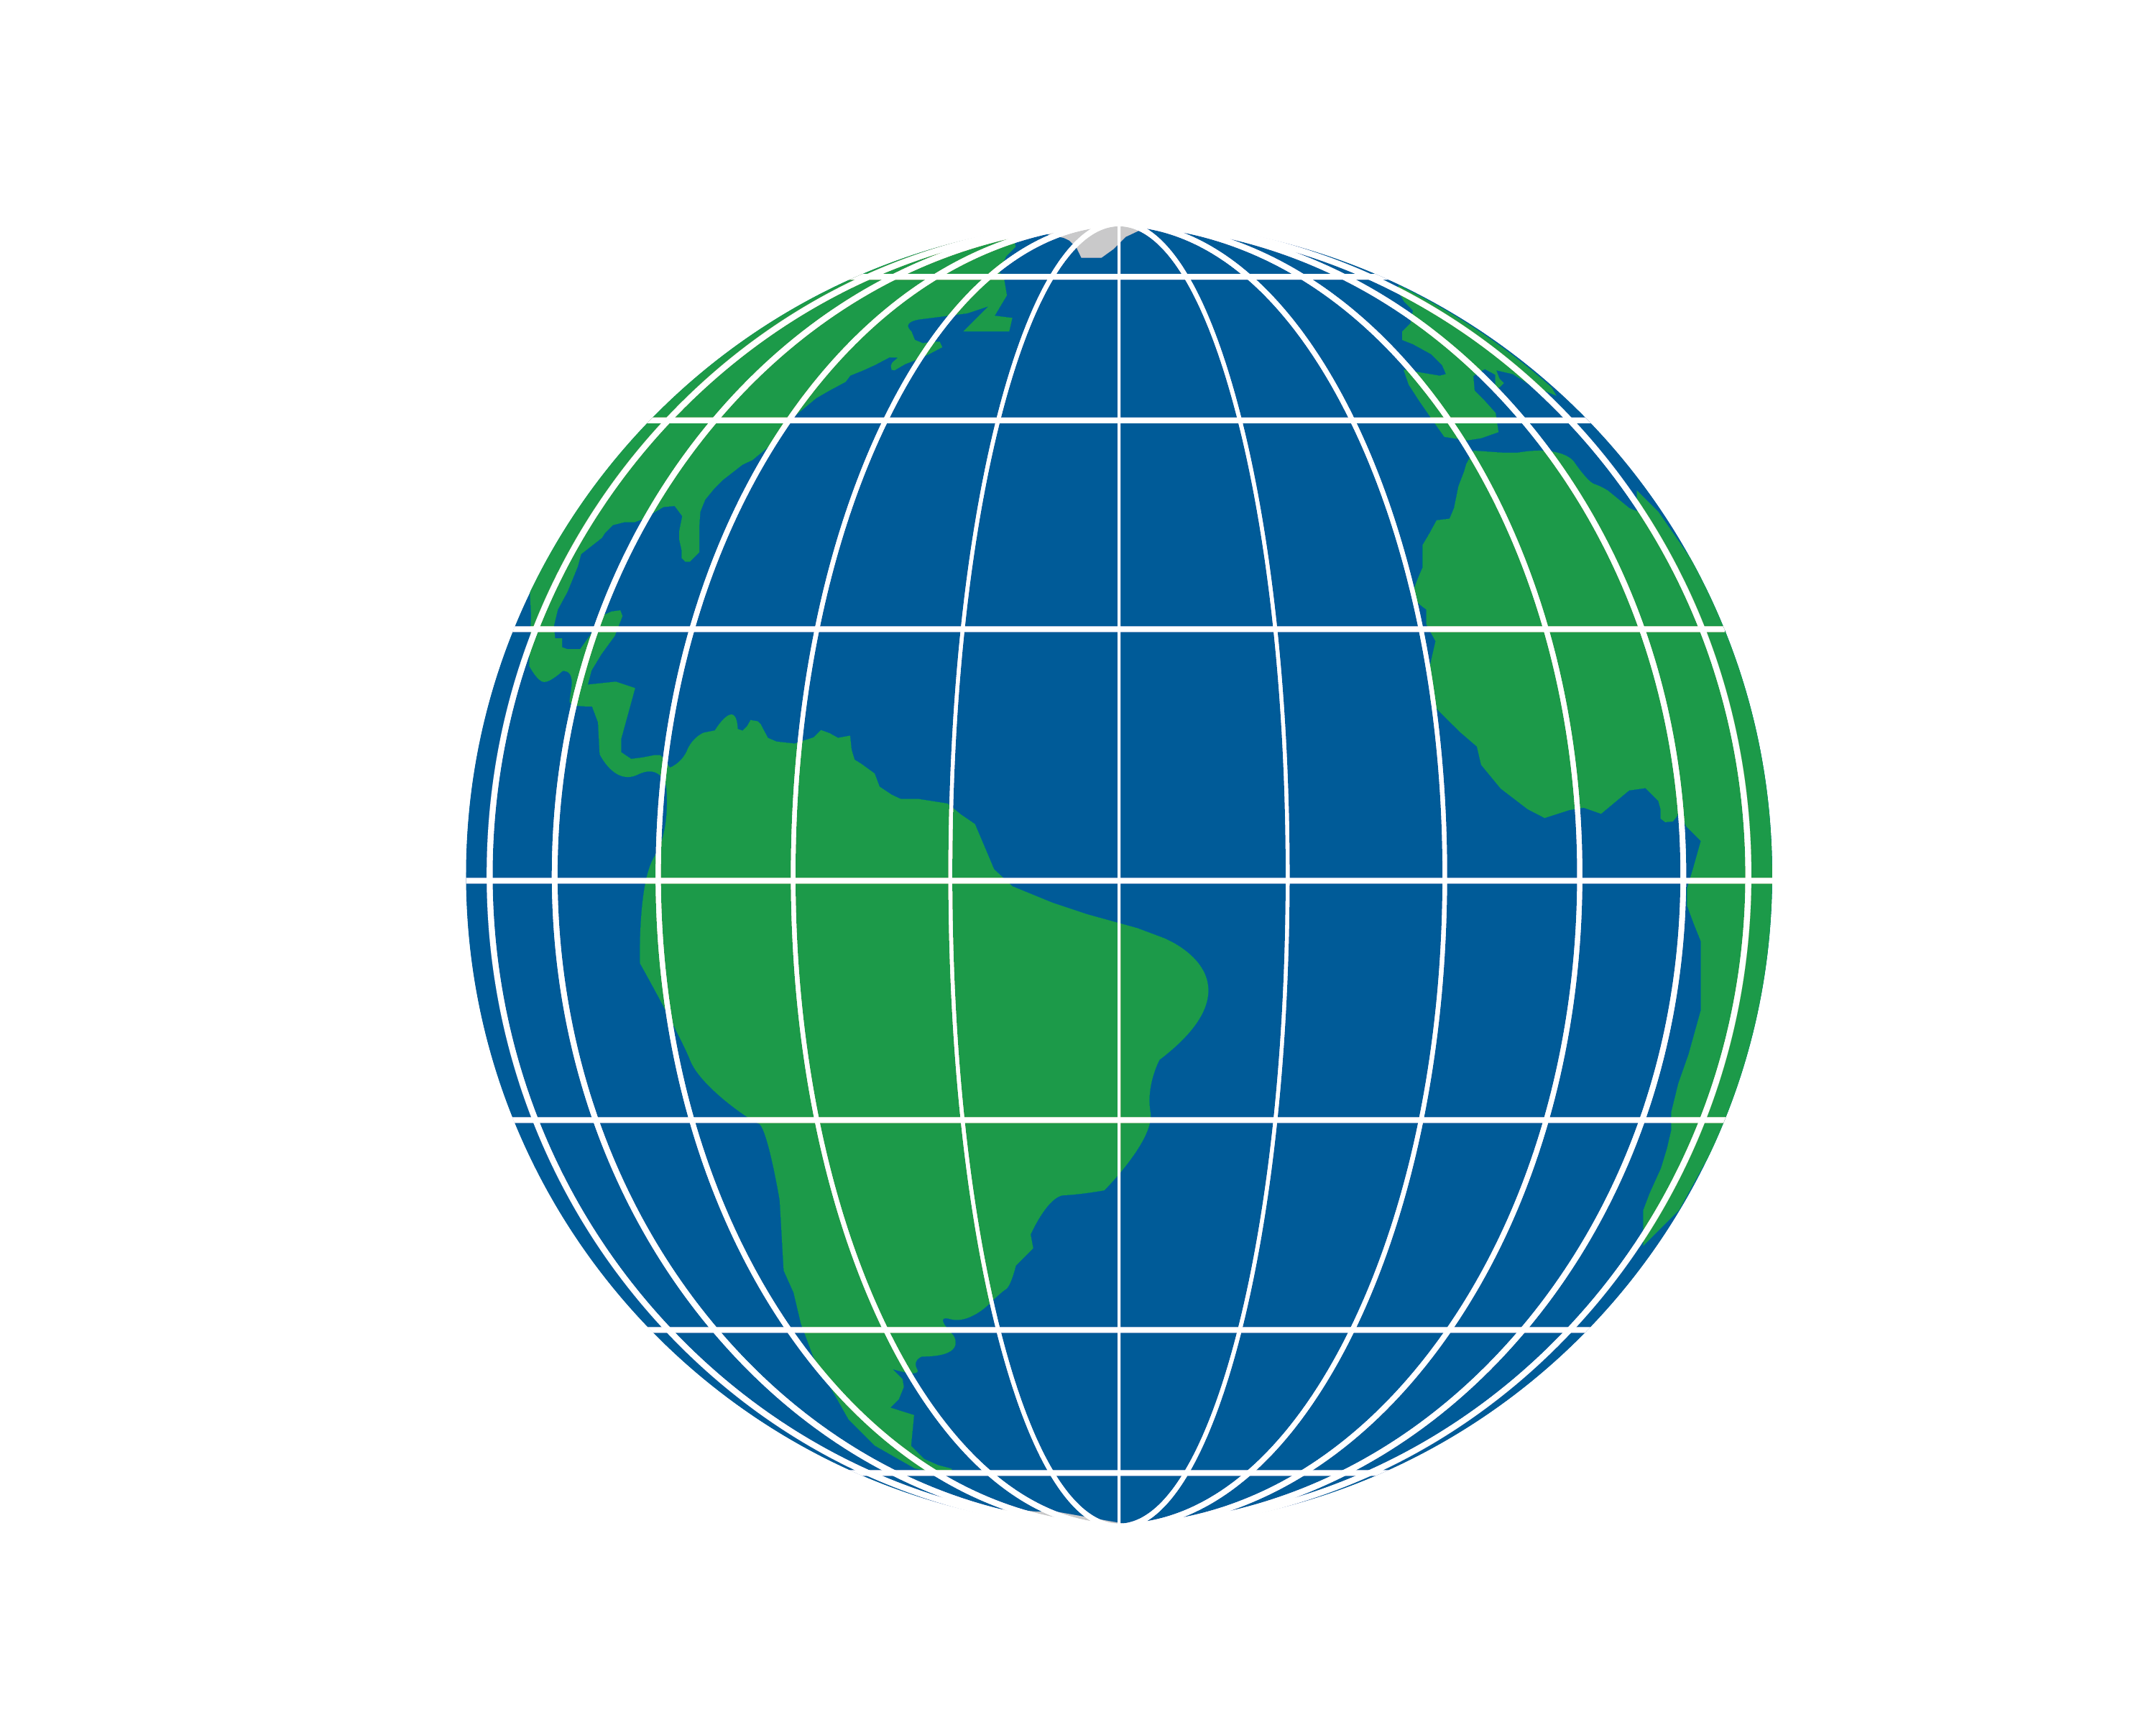
\includegraphics[width=.75\textwidth]{latLon.png}


Latitude is a measure of a point's distance north or south of the
Equator, expressed in degrees. It ranges from $-90^{\circ}$ at the
South Pole to $+90^{\circ}$ at the North Pole, with $0^{\circ}$
representing the Equator.

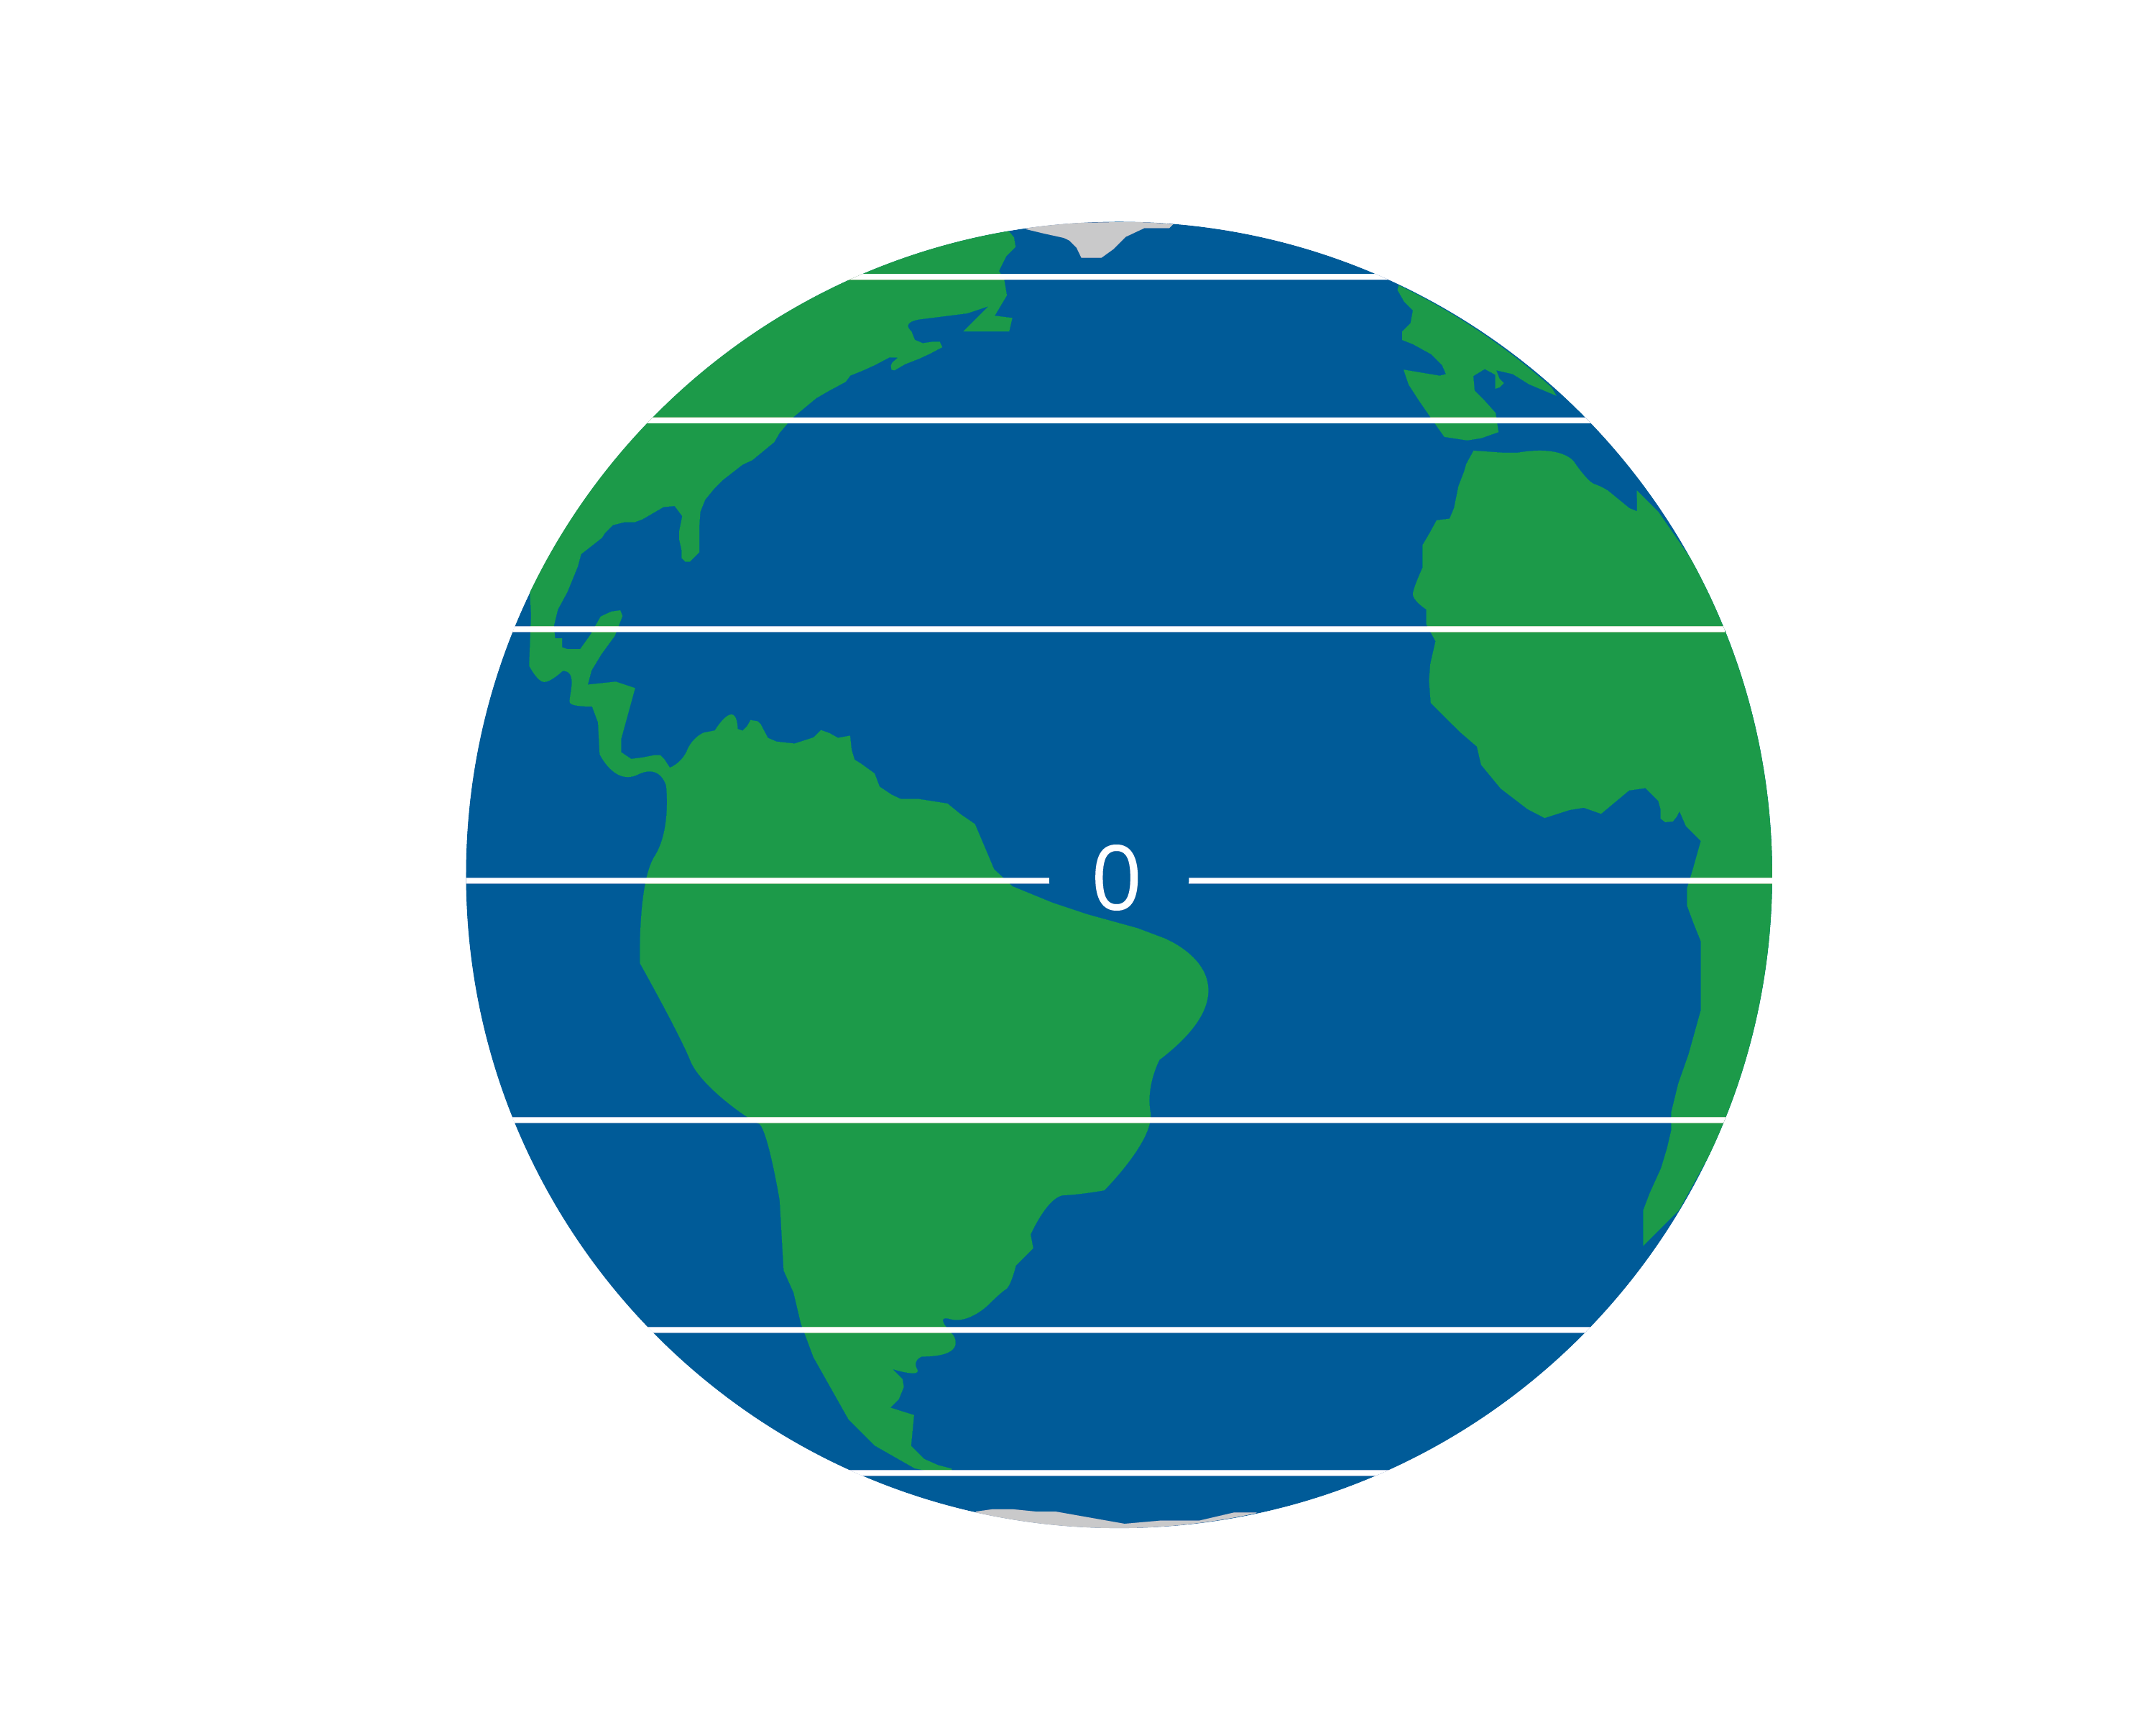
\includegraphics[width=.75\textwidth]{lat.png}

Longitude, on the other hand, measures a point's distance east or west
of the Prime Meridian (which passes through Greenwich, England). It
ranges from $-180^{\circ}$ to $+180^{\circ}$, with the Prime Meridian
represented as $0^{\circ}$.

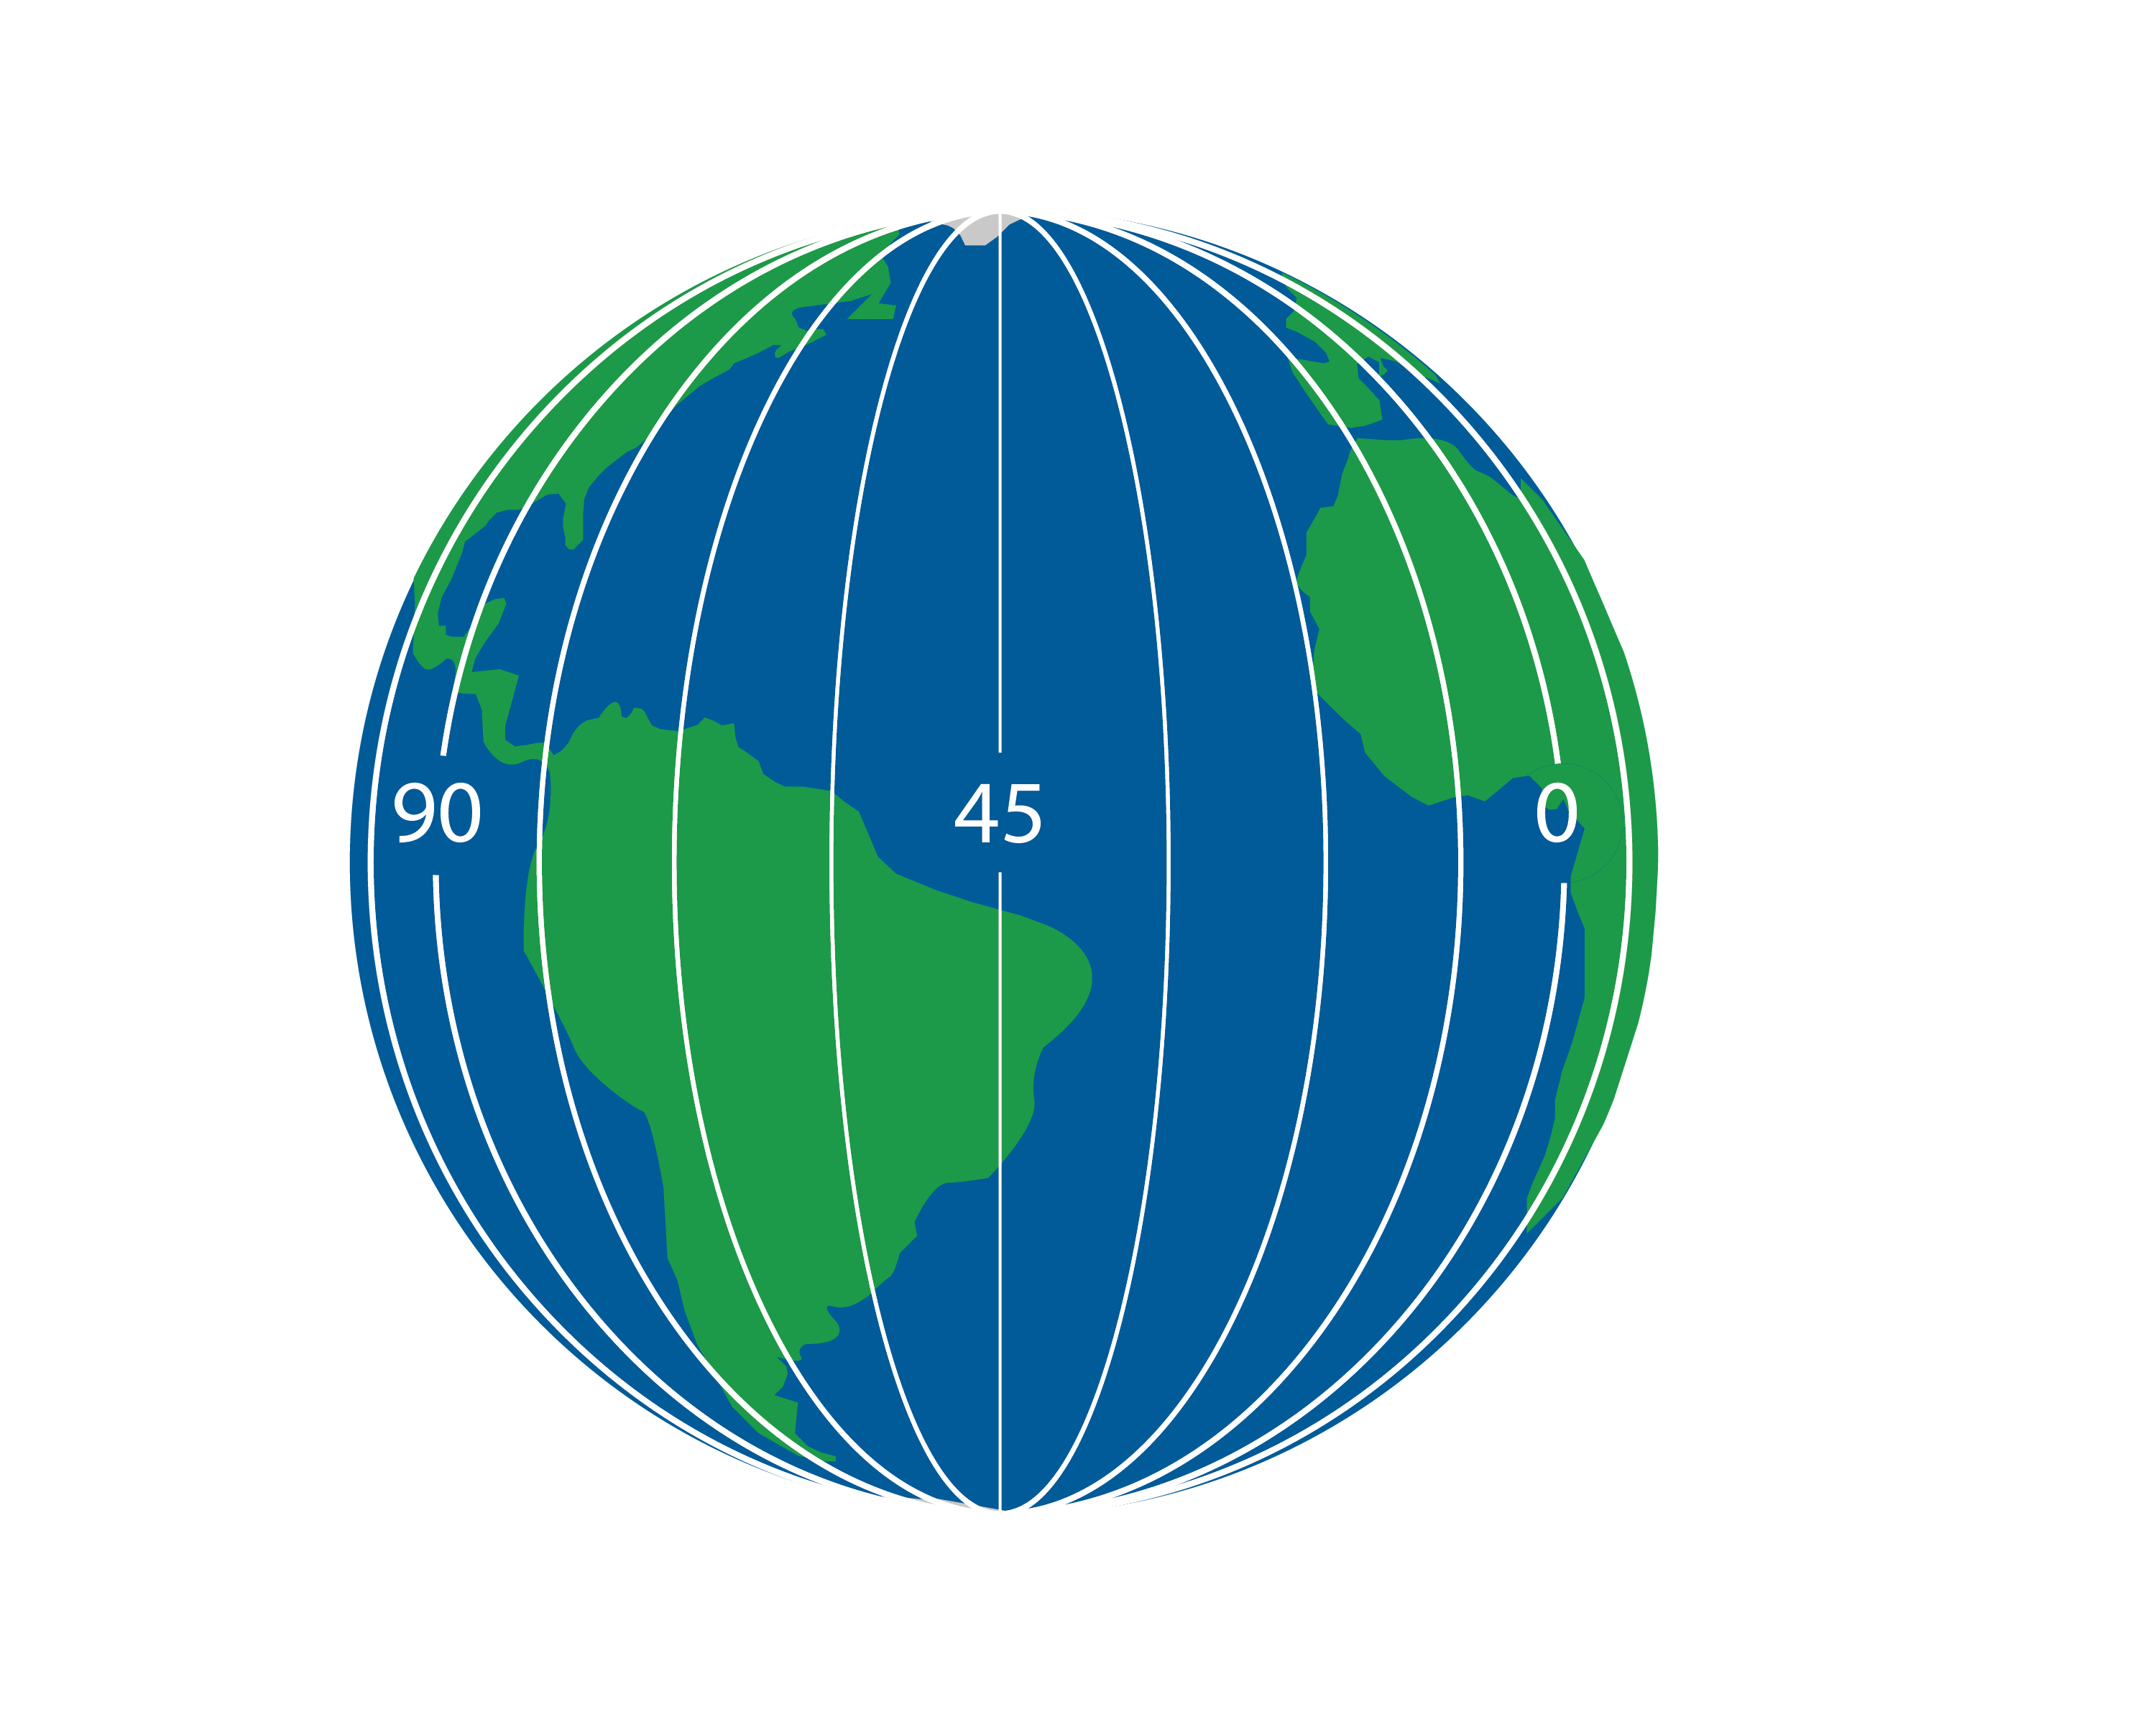
\includegraphics[width=.75\textwidth]{long.png}

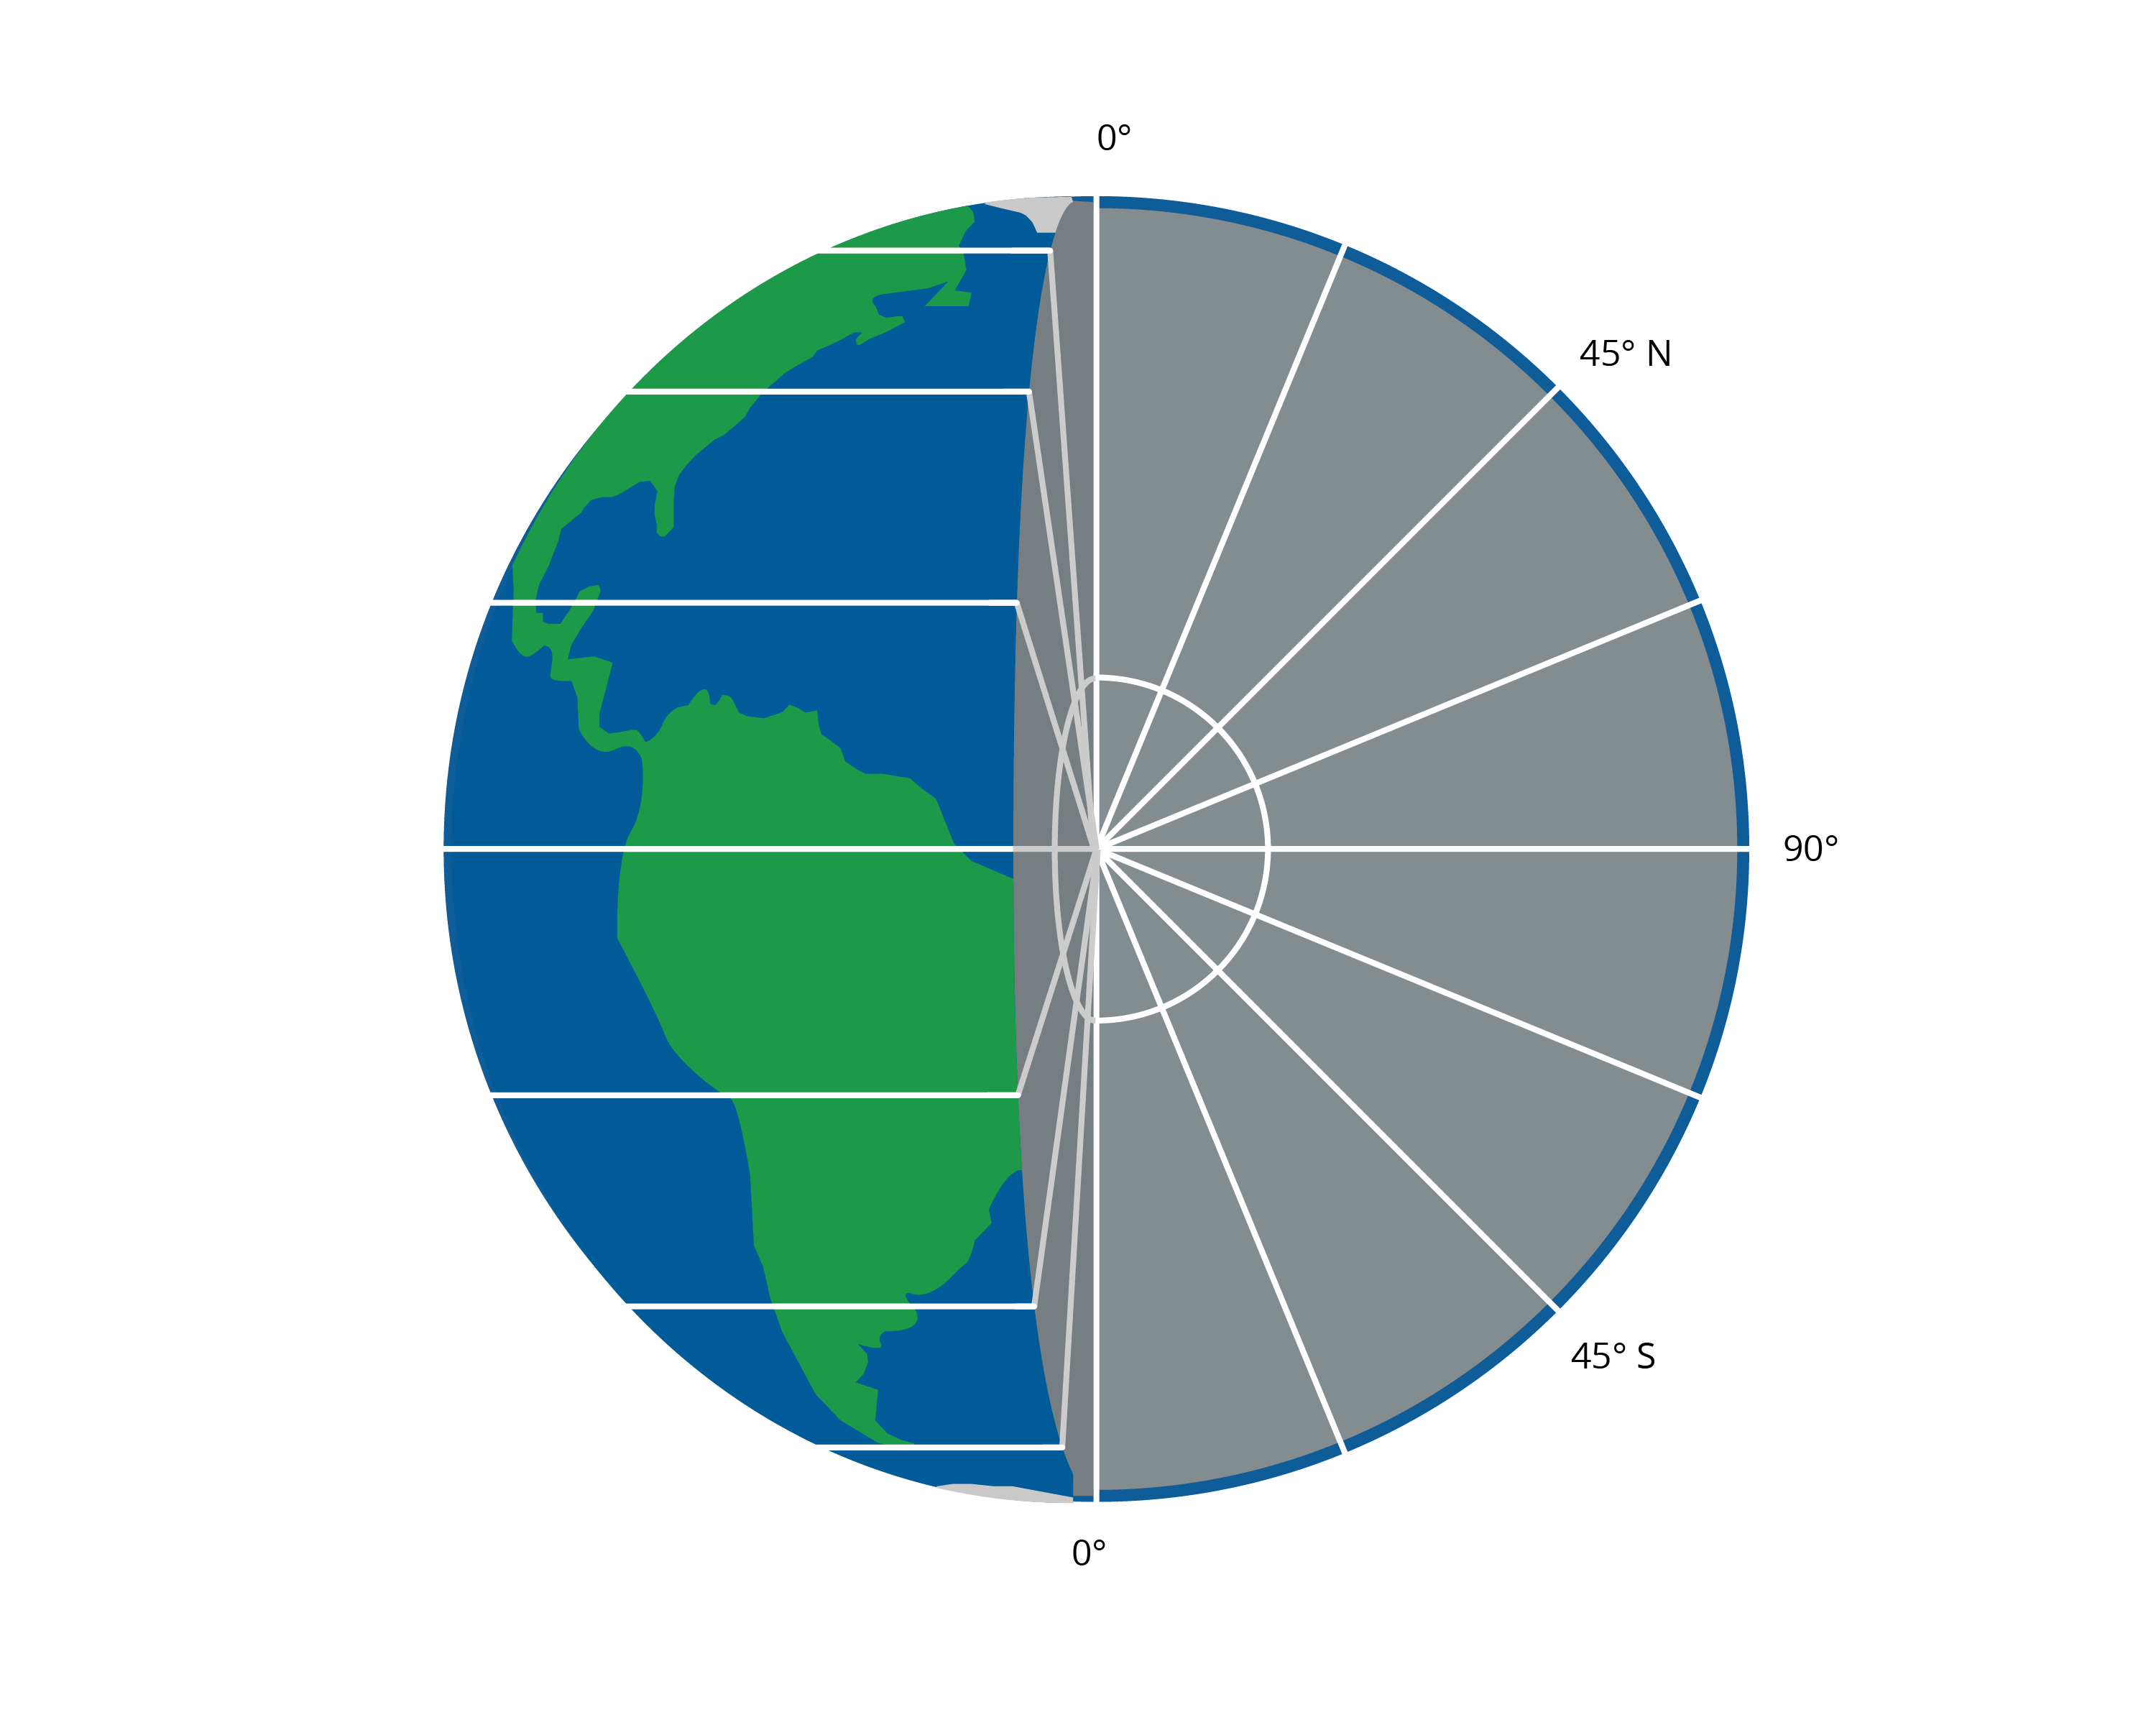
\includegraphics[width=.75\textwidth]{latExplanation.png}

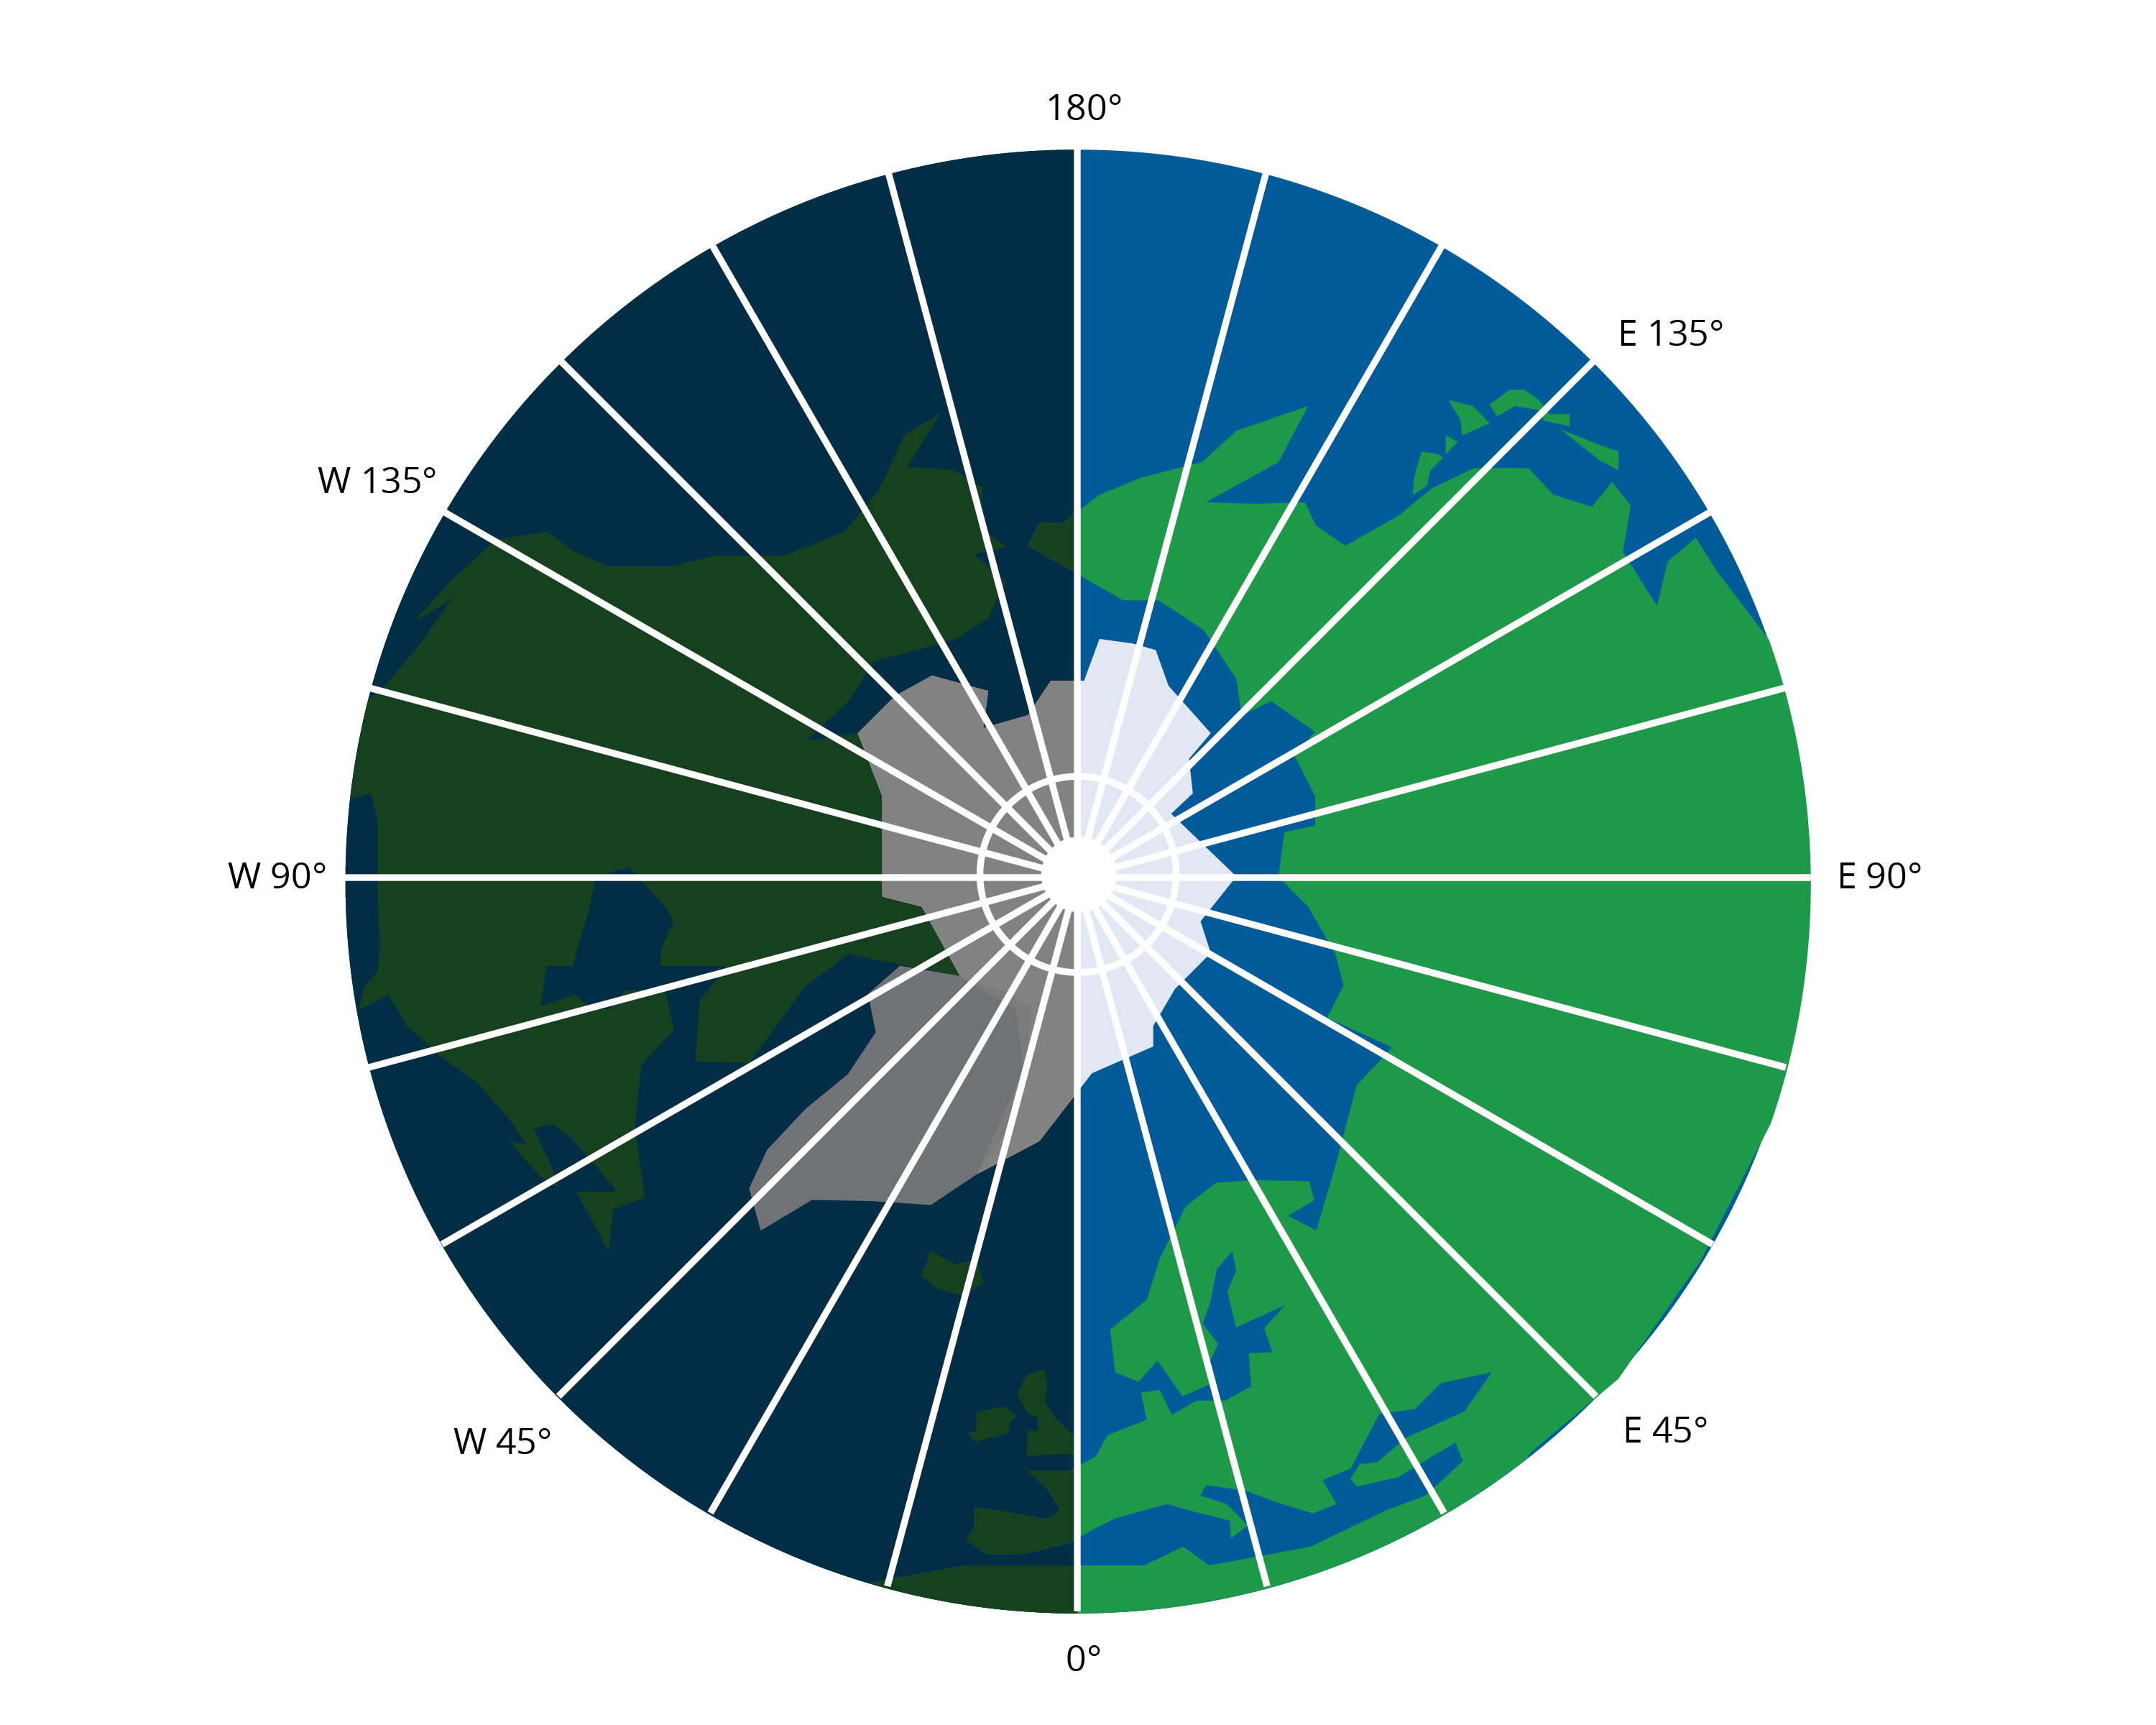
\includegraphics[width=.75\textwidth]{longExplanation.png}


\section{Nautical Mile}

A nautical mile is a unit of measurement used primarily in aviation
and maritime contexts. It is based on the circumference of the Earth
and is defined as one minute ($1/60^{\circ}$) of latitude. This makes
it directly related to the Earth's geometry, unlike a kilometer or a
mile, which are arbitrary in nature. The exact value of a nautical
mile can vary slightly depending on which type of latitude you use
(e.g., geodetic, geocentric, etc.), but for practical purposes, it's
often approximated as 1.852 kilometers or 1.15078 statute miles.\index{nautical mile}

\section{Haversine Formula}

The haversine formula is an equation important in navigation for
giving great-circle distances between two points on a sphere from
their longitudes and latitudes. It's especially useful when it comes
to calculating distances between points on the surface of the Earth,
which we represent as a sphere for simplicity.\index{Haversine
  formula}

  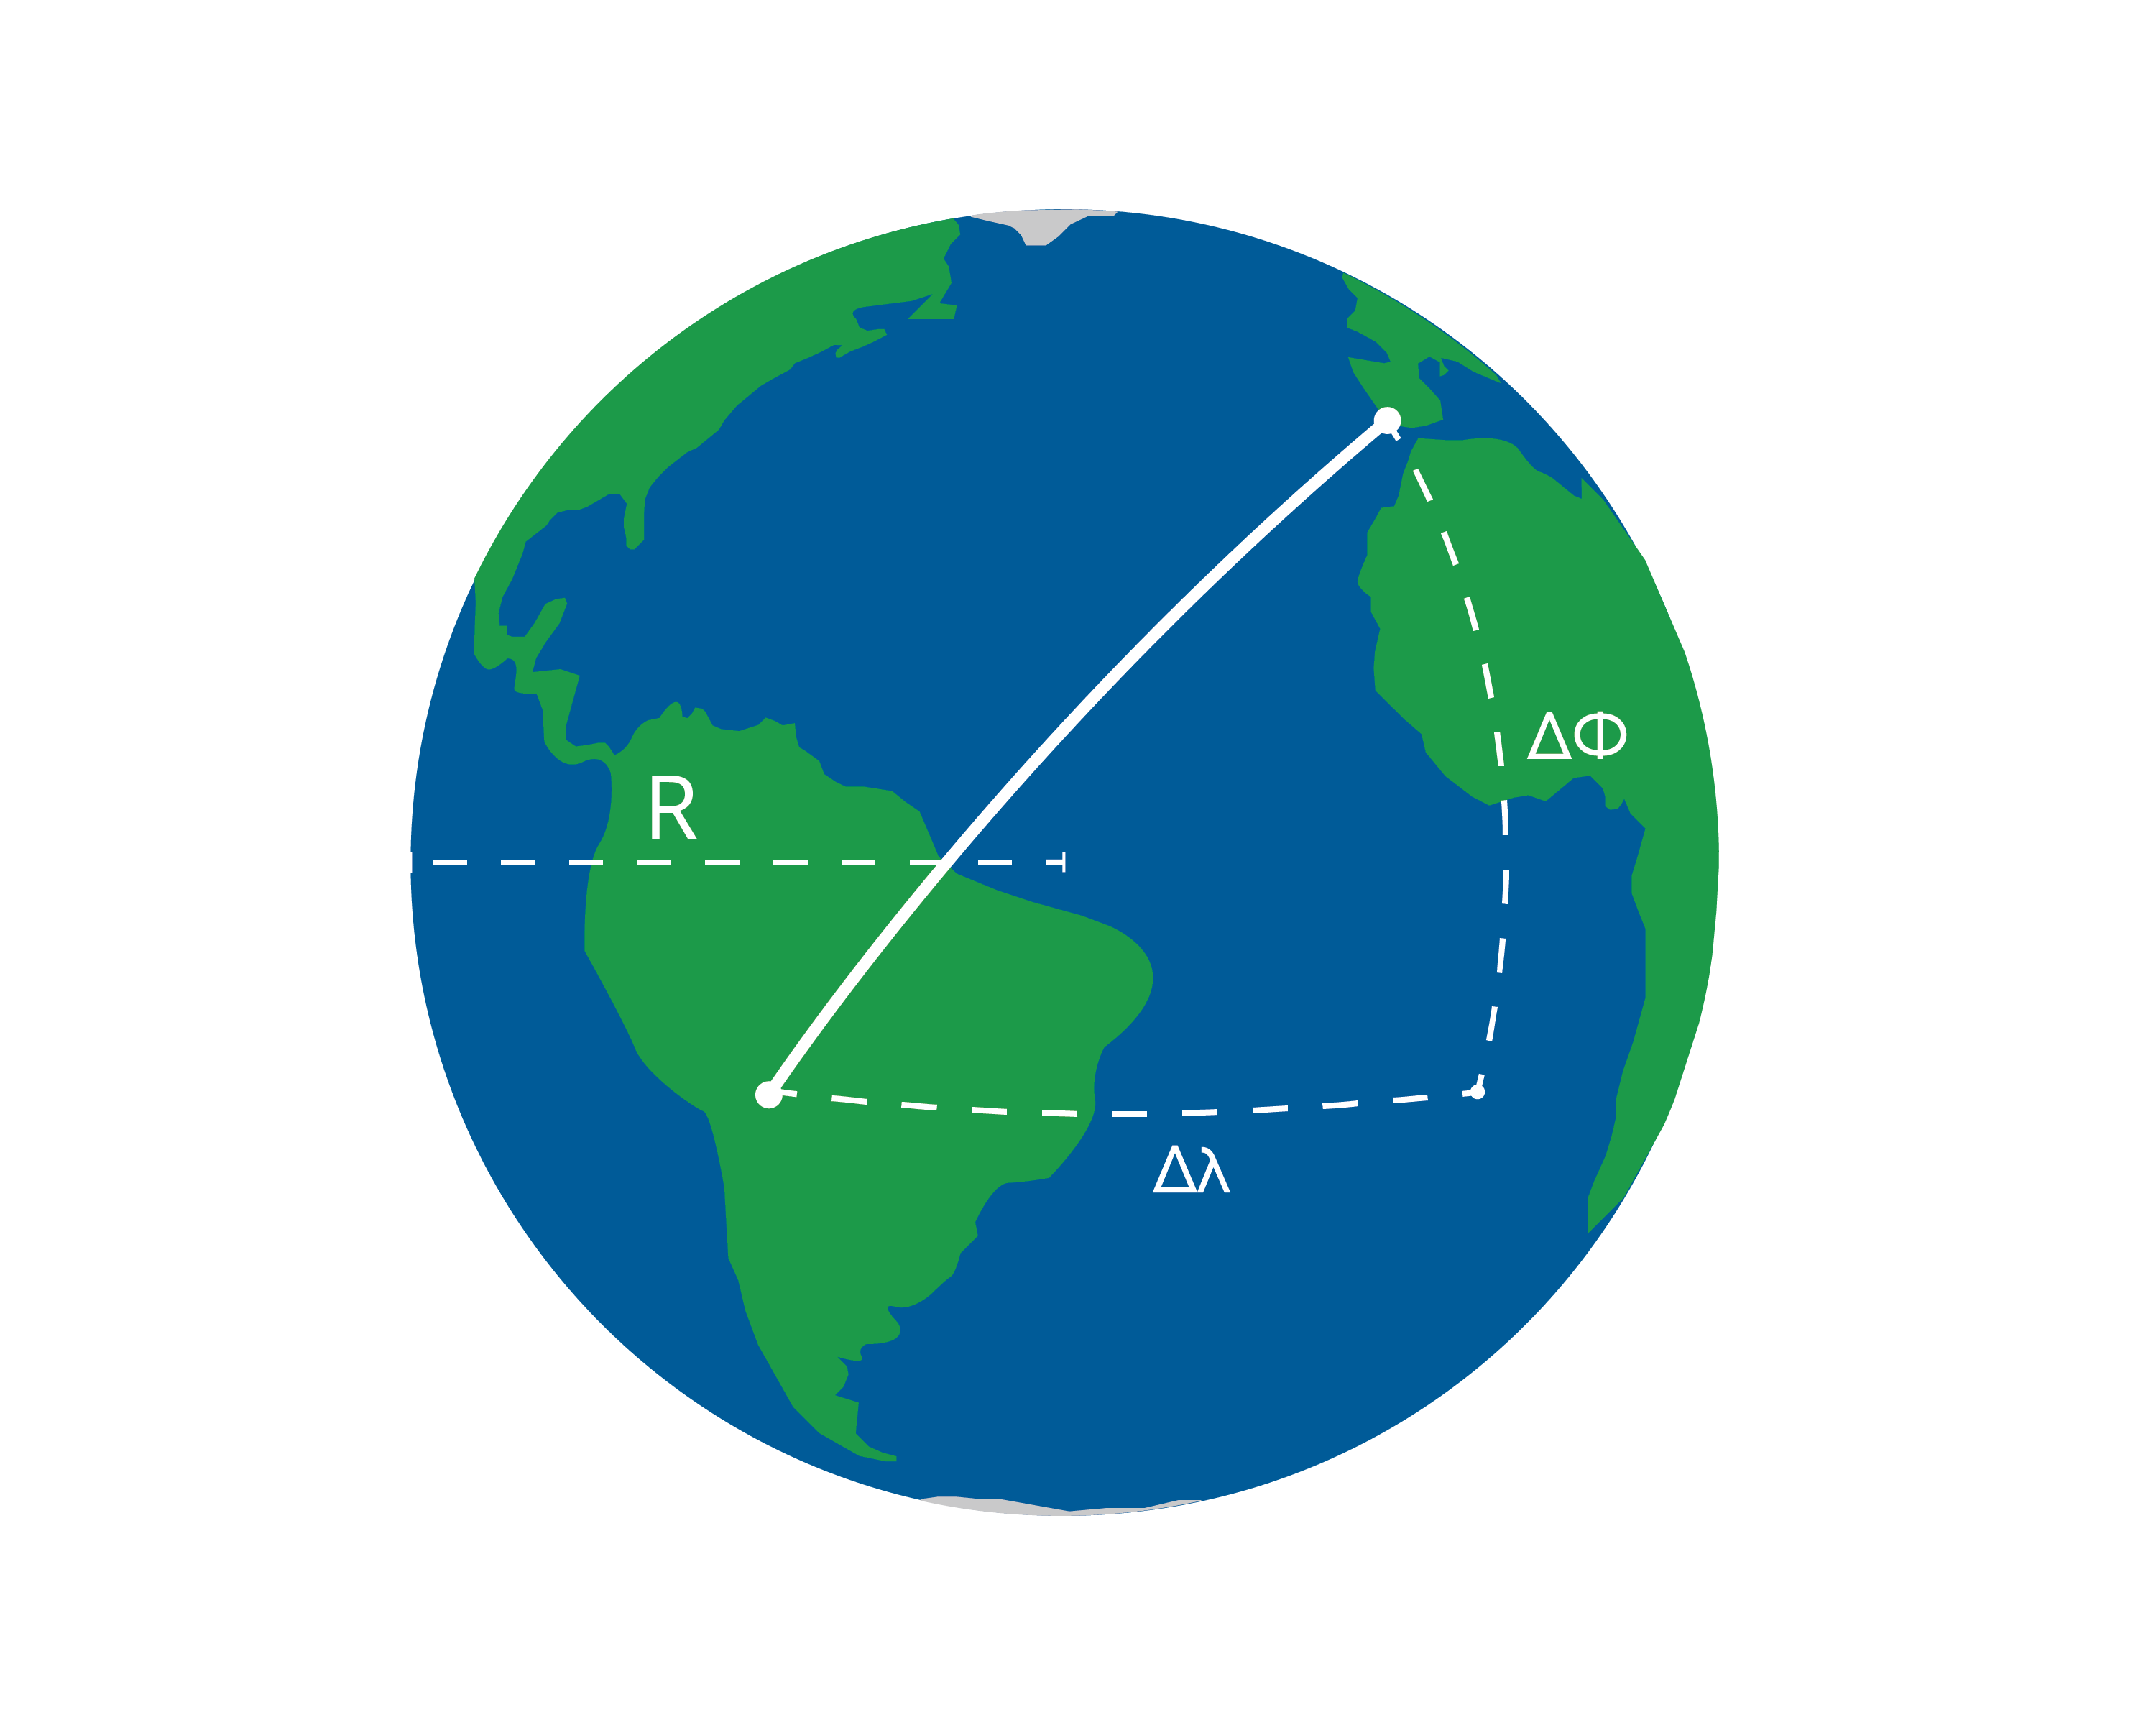
\includegraphics[width=\textwidth]{haversine.png}


In its basic form, the haversine formula is as follows:

\[
a = \sin^2\left(\frac{\Delta\phi}{2}\right) + \cos(\phi_1)\cos(\phi_2)\sin^2\left(\frac{\Delta\lambda}{2}\right)
\]

\[
c = 2 \cdot \text{atan2} \left( \sqrt{a}, \sqrt{1-a} \right)
\]

\[
d = R \cdot c
\]

Here, $\phi$ represents the latitudes of the two points (in radians),
$\Delta\phi$ and $\Delta\lambda$ represent the differences in latitude
and longitude (also in radians), and $R$ is the radius of the
Earth. The result, $d$, is the distance between the two points along
the surface of the sphere.
